\chapter{Getting Started}

\section{What is an Arduino?}

At its simplest an Arduino is a tiny computer.
Unlike personal computers which hide their internals to prevent them from being damanged
Arduinos expose all their wiring to the outside world.
While your laptop can only use USB to communicate with outside devices
an Arduino can send and receive binary voltage signals.
This ability makes an Arduino an ideal platform for physical programming.
For example in the CCHS workshop Arduinos are used to control the small C\&C mill, the laser cutter and all the 3D printers you see.

At a more technical level the Arduino is an 8bit \textbf{micro controller} 
placed on a printed circuit board which safely exposes all the pins of the chip. 
There is already a primitive operating system on the chip which any software you write will interface with.
This makes writing software much easier as you only need to explicitly control the hardware which you want to,
for example writing and uploading your first program 
to blink an LED 
will take about 5 minutes,
doing the same for a naked micro controller would take about 6 weeks in an introductory university course.

The real strength of the Arduino comes from using \textbf{shields},
these are custom designed modular circuit boards which fit on top of the Arduino
and each other.
They range complexity from safe high current switches all the way up to working gsm modules which allow the Arduino to be controlled by sms.
Each comes with custom software which allows them to ``just work'' with the Arduino.

You won't be using shields in this tutorial since each shield has it's own quirks and gotchas that only distract you from learning the basics of the Arduino that are universal across all projects.


\subsection{Uploading}
Getting the Arduino to work with your personal computer takes some effort and is different for every computer.
The CCHS Arduinos are already set up to work with the CCHS Windows laptops,
and the software which you will use are already installed on the laptop.

If you wish to use your own computer then the rest of this section will not work for you.
You can copy the examples from this tutorial directly from the software appendix.

After the computer starts there maybe some updates that need to be installed.
Leave them running for a few minutes,
if it takes more than that ask someone to check on the computer.

Before you do anything else connect the Arduino and laptop using the provided USB cable: 

\begin{center}
    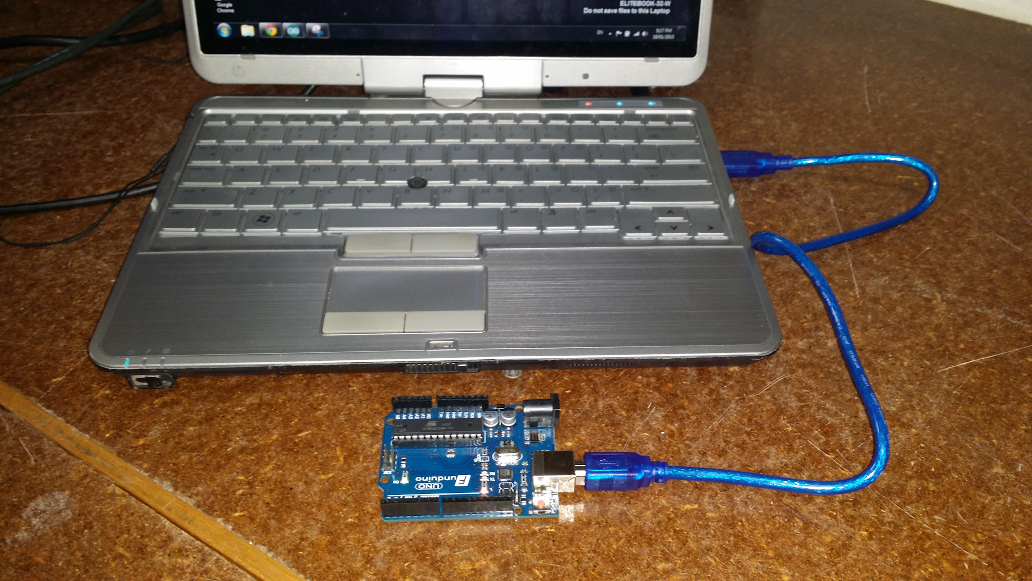
\includegraphics[width=0.4\textwidth]{./Graphics/usb_connection}
\end{center}

Next launch the 
\textbf{Arduino Integrated Development Environment (IDE)}
by clicking its icon on the desktop. 

\begin{center}
    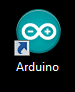
\includegraphics{./Graphics/arduino_icon}
\end{center}

The Arduino IDE will then launch with an empty project.

\begin{center}
    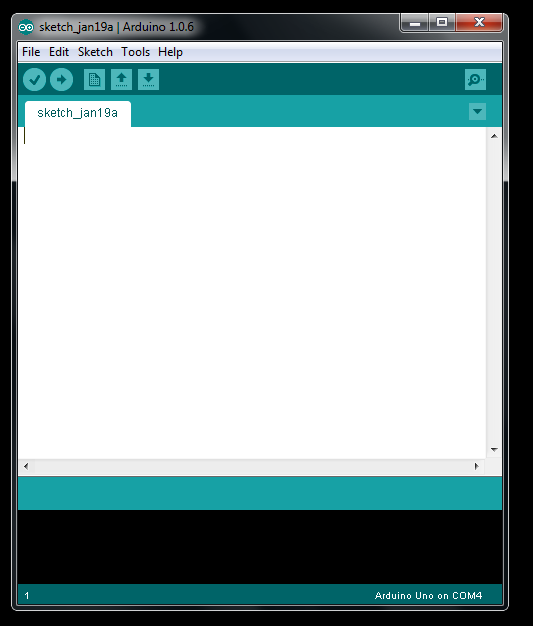
\includegraphics[width=0.4\textwidth]{./Graphics/ide_start}
\end{center}

To check that everything works fine with the IDE and Arduino we will upload a program,
called a \textbf{sketch},
to the Arduino.
The most basic sketch is \lstinline|Blink|
as the name suggests it blinks something on the Arduino.
You can find it under: 
\lstinline|File>Examples>00.Hack>Blink|.

\begin{center}
    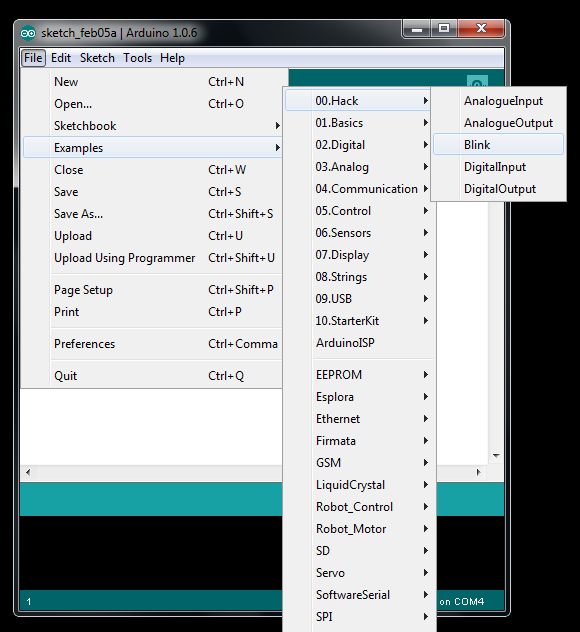
\includegraphics[width=0.4\textwidth]{./Graphics/ide_blink}
\end{center}

A new window with some code should open.  
We are not interested in the code right now,
just in getting the sketch running on the Arduino.

To upload the sketch click on the highlighted arrow button. 
The IDE will think for a bit and seem to do nothing.
When it has finished uploading the sketch a \lstinline|Done Uploading|
message will appear underneath the code
along with some technical details.

\begin{center}
    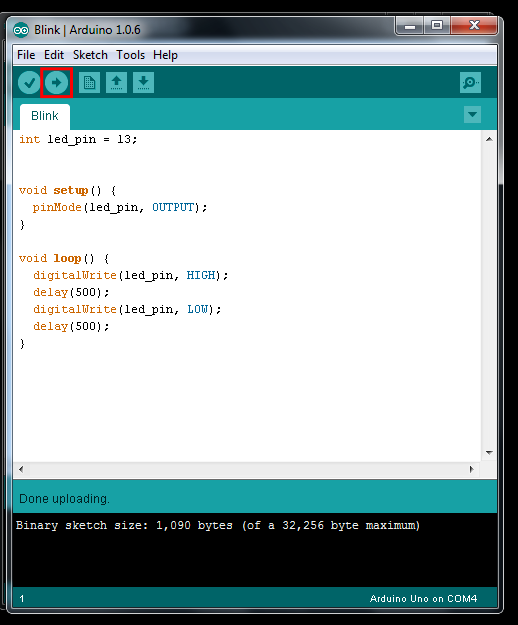
\includegraphics[width=0.4\textwidth]{./Graphics/ide_upload}
\end{center}

If everything worked you will now see the highlighted LED,
labeled L on the Arduino,
blinking once a second.


\begin{center}
    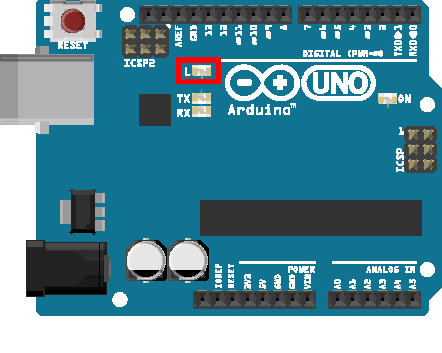
\includegraphics[width=0.4\textwidth]{./Graphics/arduino}
\end{center}

Congratulations!
You just got your first Arduino program running!

If it didn't and there was an error message than most likely Windows has 
guessed that the Arduino is connected on the wrong COM port,
it should be connected on COM 4,5 or 6 depending on where it was plugged in.
If you don't know what that means ask someone for help,
don't worry we are a friendly bunch :-)


\subsection{The Blink Sketch}

This sketch has three parts, 
the declarations at the top,
the setup and loop.
Of setup and loop are universal to every Arduino sketch.

The \lstinline|setup| is run once when the sketch is uploaded to the Arduino,
when the reset button is pressed, or when the Arduino is powered off and on.
The \lstinline|loop| first runs right after set up has finished.
Once the Arduino has done all the instructions in the loop
it goes straight back at the top and starts over.
The name is somewhat of a giveaway.


\lstinputlisting[style=Arduino, linerange={1-1}]{./Src/blink.src}

The Arduino language is quite close to C in syntax.
You need to end every line with a semicolon or else you \textbf{will} get errors.
In the above line you declare an \lstinline|int|,
this means that you reserve an \lstinline|int| sized space in the Arduinos memory  
this means a whole number between about -30,000 to 30,000.
We then name that space \lstinline|led_pin| and set the value there to 13.

\lstinputlisting[style=Arduino, linerange={3-7}]{./Src/blink.src}

In proper C \lstinline|setup| would be a function 
and would need to be embedded in a larger \lstinline|main| function to run.
The minimum operating system already on the Arduino will take care of running the setup and loop function.

The \lstinline|void| keyword tells the Arduino that it will get
no information from the function on what it is doing.

\lstinline|pinMode| tells the Arduino to set up the hardware in such a way that pin 13 can send out strong electrical signals to the outside world.
In the CCHS Arduino pin 13 is also connected to an LED on the board,
so every time it is activated you will see the L LED turn on.
 
 \lstinputlisting[style=Arduino, linerange={8-14}]{./Src/blink.src}

 \lstinline|digitalWrite| sets a given pin either high or low,
 in this case it's pin 13.
 The \lstinline|HIGH| and \lstinline|LOW| are known as macros and come from the C programming language.
 In this case they stand for the voltages we want out of pin 13:
 0V and 4.7V respectively.
 In general macros can stand for any text you do not want to type out, or as in our case implementation details you want someone else to take care
 of somewhere.

\lstinline|delay| is function that makes the Arduino wait for a given time in thousands of a second.
In this case 500, or half a second.
